
\subsection{Ring-LWE}\label{ring-lwe}
One of the recurring problems in lattice-based cryptography is the key-size and general efficiency. In the GGH cryptosystem, the key-size is $\tilde{O}(n^4)$. In the system based on the hardness of LWE presented in the previous section, the size is in the range of $\tilde{O}(n^2)$\footnote{There are $m$ samples of length $n$. Turns out that for $m > n$, the problem can become only easier, but the same holds for $m \ll n$. Therefore, in most applications, $m$ is chosen to be roughly the size of $n$.}. As we will also see later, there is some minimal efficiency needed for the scheme in order to enable the boostrapping (for FHE). Unfortunately, none of the schemes presented so far satisfy those criterions and so, we need to look for something better.

One idea to improve the efficiency, is to assume some underlying structure of the space we are performing computations in. For example, we can assume that the $\bm{a}$ vectors from previous section are given to us in block of $n$ samples $\bm{a}_1, \bm{a}_2, \dots, \bm{a}_n \in \Z_q^n$ where all of the elements are related. Namely, $\bm{a}_1 = (a_1, \dots, a_n)$ is again chosen uniformly but each $\bm{a}_i = (a_{\mu(1)}, a_{\mu(2)}, \ldots, a_{\mu(n)})$ is a permutation by some $\mu$ of the initial $\bm{a}_1$. This choice seems rather arbitrary however we will show how it is a natural consequence of everything we did so far and yields arguably the best results. For example if $n = 4$ and $q = 17$ and $\bm{a}_1 = (1, 16, 4, 5)$ as before, then $\bm{a}_3$ could have the form $(4, 5, 16, 1)$. Note that representing $n$ vectors now takes only $O(n)$ elements from $\Z_q$ rather than $O(n^2)$. The underlying structure is a ring, hence the name ring-LWE (or R-LWE), that is, we replace the group $\Z_q^n$ by picking some ring $R$ of degree $n$ over $\Z$ and a positive modulus $q$ defining the quotient ring $R_q := R/qR$. In this exposition, to simplify some steps, $R$ is taken to be a \textit{cyclotomic} ring -- i.e. $R_q = \Z_q[x]/ (x^n + 1 )$ for $n = 2^k$ which turns out to yield much simpler proofs for somewhat weaker results.

In the year 2010, Vadim Lyubashevski, Chris Peikert and Oded Regev presented their paper ``On Ideal Lattices and Learning With Errors Over Rings'' \cite{ring-lwe}. The main purpose of the paper was to ``translate'' the LWE problem onto a ring as was done with the SIS problem (mainly by Micciancio \cite{ring-sis} that was followed up by other works but these results are not presented in this paper) and followed the heuristic approach behind the NTRU\footnote{As mentioned by Peikert in his survey: ``The meaning of the acronym NTRU is somewhat mysterious; plausible candidates include "$N$th degree \textit{tru}ncated polynomial ring" and "Number Theorists ’R’ Us."'' -- \cite{lattice-survey}} cryptosystem \cite{ntru}. This in particular means first, defining the ring-LWE and later proving the hardness based on some difficult lattice problems like \prob{SVP} along with pseudorandomness of the ring-LWE distribution (analogous to \ref{s-to-d} whose definition will appear later). The second issue turned out to be quite nontrivial and required good insight in the algebraic number theory as well as Gaussian measures and distributions. This is finally where we can use all the theory developed in the Section \ref{ant} on algebraic number theory.

Somewhat analogous to the previous section, this one is also split into two main parts. First part - Section \ref{h-rlwe} -- focuses on the hardness of the search version of the RLWE. The approach is identical to the one presented for the standard LWE. However, one needs to pay attention to details that are implied by the shift to $R$ like for example the shape of the error distribution under the canonical embedding. Fortunately for us, the quantum part of the reduction can be adopted almost as is and so, we will only mention it briefly. The second part -- Section \ref{pseudo-rlwe} -- deals with pseudorandomness of the RLWE distribution and thus proving the equivalence between the search and decision versions. This one will require much more insight into the algebraic number theory compared to any other part of this paper and so, we will discuss it in much more detail. Before we dwell any further, we need to establish some terminology and useful lemmas. This is done in the following section.

\subsubsection{Preliminaries}
In this section we will formally introduce the underlying ring structure that will be used throughout this section. We will try to spell out in more detail facts and results that are used implicitly in the original \cite{ring-lwe} providing few examples along the way. Most of those results will mainly be useful for the second part which is the decision to search reduction. In the first part, the hardness of search version, holds for any number field, not necessarily cyclotomic.

Let us therefore fix a cyclotomic number field $K$ of degree $n$. More precisely, if we take $m = 2^k$ for some $k \geq 2$ and set $n = \phi(m) = m/2 = 2^{k-1}$, then by Corollary \ref{2k-cycl} we obtain
\[ K := \Q[x]/\Phi_m(x) = \Q[x]/(x^n + 1) \cong \Q(\zeta), \]
where $\zeta = \exp(2 \pi \sqrt{-1}/m)$ is the $m$-th root of unity. We define our initial ring to be
\begin{equation} R := \Oo_K = \Z[\zeta] \end{equation}
where the equality holds by Proposition \ref{cycl-ok} and therefore is generated by $\{1, \zeta, \dots, \zeta^{n-1} \}$. Recal at this point the notion of the dual lattice in a number field. It is all the elements $\alpha \in K$ such that $\Tr_{K/\Q}(\alpha R) \subset \Z$. By Equation \ref{d-basis}, the basis for 

This ring however is slightly too big for our desire. Analogously to the LWE case we therefore consider the coset obtained by reducing all elements modulo some integer $q$. This gives us the final form of the underlying ring as 
\begin{equation} R_q = R/qR = \Oo_K/q \Oo_K = \Z_q[\zeta]. \end{equation}
\subsubsection*{Ideal Lattices}
Let us now spell out few nice properties of $R$ and $R_q$ and introduce the ideal lattices. For a good discussion on the \textit{different} ideal, see Keith Conrads \href{https://kconrad.math.uconn.edu/blurbs/gradnumthy/different.pdf}{paper}.

Recal the notion of fractional ideals and their inverses from Section \ref{ant}. They are ideals $\I$ of $K$ such that there is some $\alpha$ such that $\alpha \cdot \I \subset \Oo_K$. When embedden in $\C^n$, they yield us lattices which we call \textit{ideal lattices}. We ilustrate these concepts with a small example.
\begin{example}
	Take $K = \Q(\sqrt{-1})$ the fourth cyclotomic field. Its ring of integers is $\Oo_K = \Z[\zeta_4] = \Z[\sqrt{-1}]$ by Proposition \ref{cycl-ok} and is spanned by $\{1, \sqrt{-1}\}$. The canonical embedding into $\C^2$ is therefore given by
	\begin{align*}
    a + b\sqrt{-1} \mapsto & (a + b\sqrt{-1}, a - b\sqrt{-1}) = \\
						   & a (1,1) +  b(\sqrt{-1}, -\sqrt{-1}),
 	\end{align*}
	and is shown in Figure \ref{fig:embed}. For convenience, denote $\bm{b}_1 = \sigma(1) = (1,1)$ and $\bm{b}_2 = \sigma(\sqrt{-1}) = (\sqrt{-1}, \sqrt{-1})$. Let us now see how some ideal $\I = (1 + 2\sqrt{-1})$ embeds. A general form of an element $\alpha \in \I$ is a multiple of $1 + 2\sqrt{-1}$ so we compute 
	\[(a +b\sqrt{-1})(1+2\sqrt{-1}) = a(1+2\sqrt{-1}) + b(-2 \sqrt{-1})\] for $a,b \in \Z$. The elements $1+2\sqrt{-1}$ and $-2 + \sqrt{-1}$ form a basis for $\I$. The $\sigma(\I)$ is determined by the embedding of its basis so we compute $\sigma(1+2\sqrt{-1}) = (1+2\sqrt{-1}, 1+2\sqrt{-1})$ and $\sigma(-2 + \sqrt{-1}) = (-2 +\sqrt{-1}, -2 -\sqrt{-1})$. We now have
	\[ \sigma(\I) = \{a(1+2\sqrt{-1}, 1+2\sqrt{-1}) + b (1+2\sqrt{-1}, 1-2\sqrt{-1}) : a,b \in \Z \} \subset \sigma(\Oo_K) \subset \C^2. \]
	%If we now express the basis of $\sigma(\I)$ with the basis of $\sigma(\Oo_K)$ we obtain the matrix
\end{example}
	\begin{figure}[ht]
    \centering
    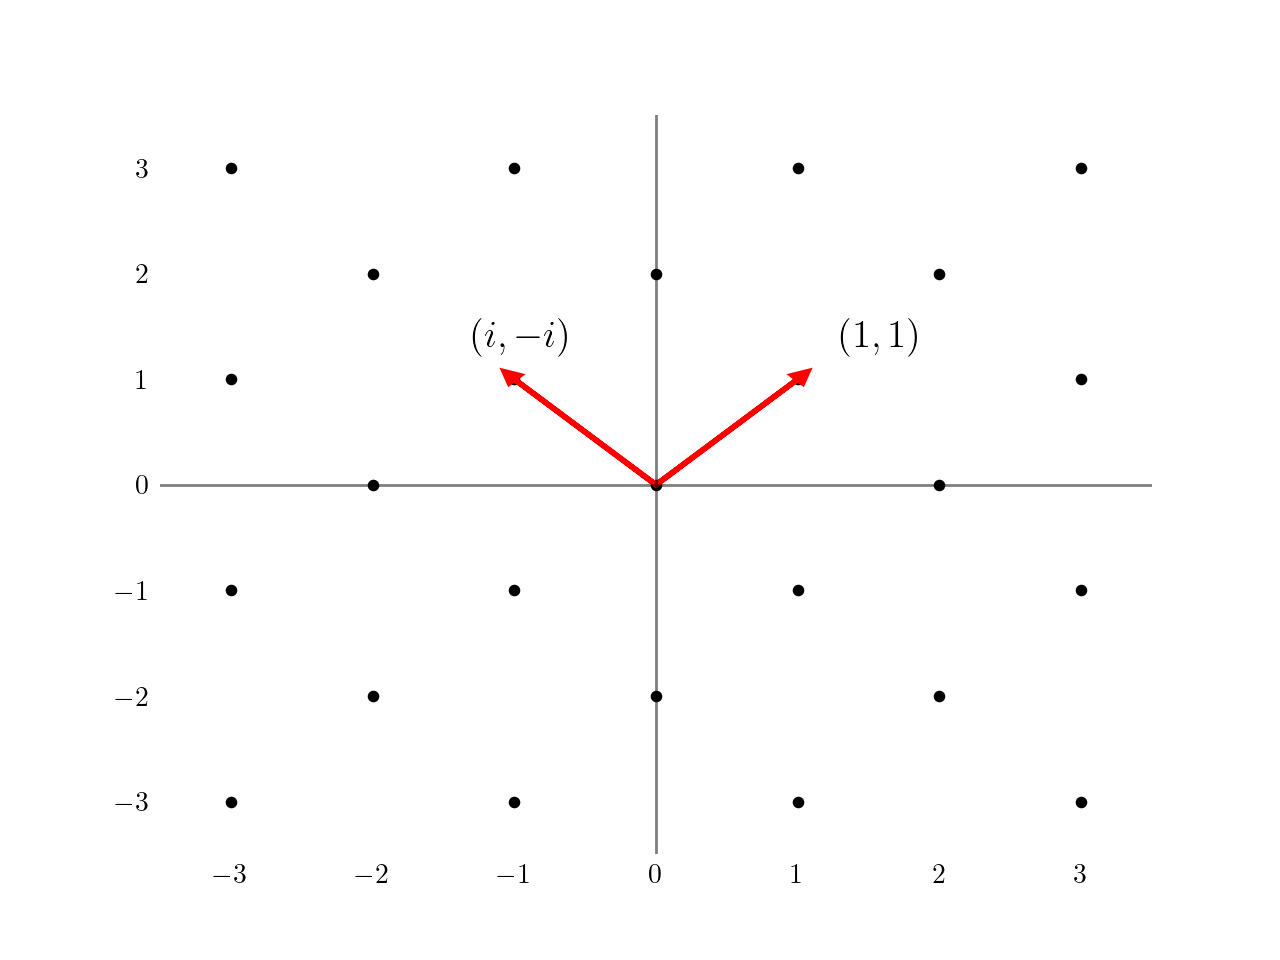
\includegraphics[scale=0.8]{images/ex_lattice.png}
    \caption{Canonical embedding of $\Z[\zeta_4]$.}
    \label{fig:embed}
\end{figure}

Let us now compute the dual of $R$. For the field $K$ is the $m$-th cyclotomic number field with $m = 2^k$, recall that the minimal polynomial of $\zeta_m$ is $x^n+1$ for $n = m/2 = 2^{k-1}$ by Proposition \ref{2k-cycl}. Then, we can use Proposition \ref{d-basis} to find the basis for the dual of $\Oo_K$. We thus compute the derivative of $f(x) = x^n +1$:
\[1/f'(x) = n^{-1} \cdot x^{1-n} \] and if we plug in $\zeta := \zeta_m$ for $x$ we obtain
\[1/f'(\zeta) = n^{-1} \cdot \zeta^{1-n}.\]
Note now that $\zeta^{1-n} = \zeta^{-n} \zeta = (\zeta^n)^{-1} \zeta = (-1)^{-1} \zeta = -\zeta$. Hence, the basis for $\Ood_K$ is given by $\{-1/n, -\zeta/n, \ldots, -\zeta^{n-1}/n \}$ which is equivalent to $n^{-1}R$.

\paragraph{Chinese Remainder Theorem}
Lastly, we will present the Chinese Remainder Theorem for rings and few related propositions that will be useful for our reductions in the two following sections.

\begin{proposition}[Chinese Remainder Theorem]\label{crt}
	Let $\I_1, \ldots, \I_r$ be pairwise coprime ideals in $R$, and let $\I = \prod_{i \in [n]} \I_i$. Then there is an isomorphism of rings
	\[ R/\I \rightarrow \bigoplus_{i \in [n]} (R/\I_i). \]
\end{proposition}
This is slightly generalized Theorem II.4.12 from J.Top lecture notes for algebraic structures and the proof is almost identical with the replacement of two coprime ideals with $n$-many.

The proofs to the following propositions can be found in \cite{ring-lwe}.
\begin{proposition}
	Let $\I$ and $\J$ be ideals in $R$. There exists $t \in \I$ such that the ideal $t \cdot \I^{-1} \subseteq R$ is coprime to $\J$.
\end{proposition}

\begin{proposition}\label{sigma-t}
	Let $\I$ and $\J$ be ideals in $R$ and let $t \in \I$ be such that $t \cdot \I^{-1}$ is coprime with $\J$. Then the function $\theta_t : K \rightarrow K$ defined as $\theta_t(u) = t \cdot u$ induces an isomorphism from $R/\J R$ to $\I R/\I \J R$.
\end{proposition}

\paragraph{Why cyclotomic?}\label{why?}
As mentioned earlier, we wish to fix the degree of our cyclotomic polynomial to a power-of-two. This leads to greatly simplified proofs of some results like for example search-to-decision reduction in section \ref{pseudo-rlwe}. Nonetheless, in places where it is not necessary, we will be using arbitrary number fields, sometimes not even cyclotomic. We will now list few desirable properties of cyclotomic rings (also those of power of two) that will be useful for us later on. Let us fix $m$, $n$ and $k$ to some positive integers.
\begin{itemize}
	\item Under the canonical embedding, the cyclotomic ring $R = \Oo_K$ for $\Phi_m(x) = x^{\varphi(m)} - 1$ embeds as a lattice which in general, is not self-dual (this is only the case for $\Z^n$). Instead, its dual lattice corresponds to a fractional ideal $\Rd \subset K$ such that $R \subseteq \Rd \subseteq m^{-1}R$. In the case where $n = \varphi(m) =  2^{k-1}$ these two are actually equivalent, namely $\Rd = n^{-1}R$. 
	\item Polynomial arithmetic modulo $\Phi_m(X)$ can be performed very efficiently using slightly adjusted, classical $n$-dimensional Fast Fourier Transform -- \cite{toolkit}, \cite{swift}.
	\item In general, the smaller the shortest vector $\lambda_1(\Ll)$ is, the less secure the system. Cyclotomic fields have relatively large $\lambda_1(\Rd)$ -- \cite{oracle}.
	\item In fact, for $n = 2^k$, we have $\lambda_n(\Rd) = 1/\sqrt{n}$
	%\item They also have relatively small \textit{expansion factors} (roughly speaking it is the ratio of the size of the public key to the size of the secret key) as defined and explained in \cite{expansion}.
	\item The cyclotomic number field is a CM-field which means that we do need to differentiate between real and complex embeddings since there are only exactly $n/2$ of the complex ones. As one can imagine this can simplify some technical steps in proofs and definitions.
	%\item Cyclotomic number fields have Galois groups that ``act transitively'' on the ideals of the ring of integers. We will explain this in more details in the Subsection \ref{pseudo-rlwe}. 
\end{itemize}
Unfortunately, cyclotomic fields with degree of a power-of-two are quite rare and restrictive. Imagine that our system is deemed insecure for some large $n = 2^k$. It might so happen that the next power of two is completely impractical when implemented. We should be able to find something inbetween the two instead.
\paragraph{The RLWE distribution}
We now formally introduce the $R$-LWE distribution and related problems.
\begin{definition}[Ring-LWE Distribution]
	For $s \in R_q$ (the ``secret'') and an error distribution $\psi$ over $R_q$, a sample from the ring-LWE distribution $A_{s, \psi}$ over $R_q \cross R_q$ is generated by choosing $a \leftarrow R_q$ uniformly at random, choosing $e \leftarrow \psi$, and outputting $(a, b = a \cdot s + e)$.
\end{definition}
\begin{definition}[Ring-LWE, Search)]
	Let $\Psi$ be a family of distributions over $R_q$. The search version of the ring-LWE problem, denoted R-LWE$_{q, \Psi}$, is defined as follows: given access to arbitrarily many independent samples from $A_{s, \psi}$ for some arbitrary $s \in R_q$ and $\psi \in \Psi$, find $s$.
\end{definition}
\paragraph{Distribution}
From this point onwards, for $\alpha > 0$, we will denote by $\Psi_{\leq \alpha}$ the set of all elliptical Gaussian distributions $\D_{\bm{r}}$ (over $R_q$) where each parameter $r_i \leq \alpha$.
\begin{figure}[ht]
	\centering
	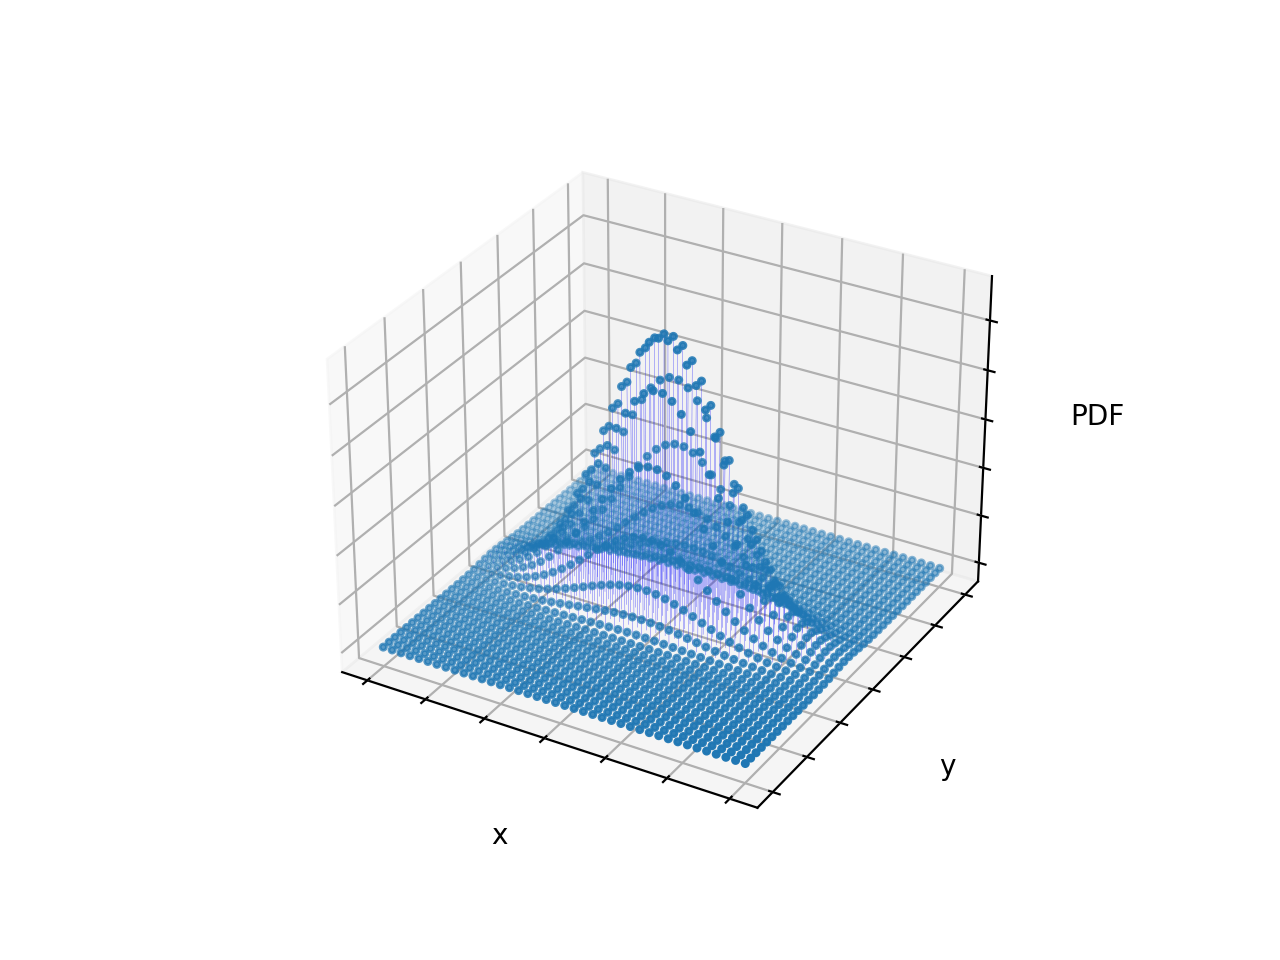
\includegraphics[scale=0.7]{elip.png}
	\caption{Eliptical Gaussian with $r_1 = 0.5$ and $r_2 = 4$. The level sets $z=k$ constitute ellipses.}
	\label{elip-gauss}
\end{figure}
\subsubsection{Hardness of search Ring-LWE}\label{h-rlwe}
We can finally discuss the main results from the \cite{ring-lwe}. This section focuses on the quantum reduction from $R$-LWE$_{q, \Psi_{\leq \alpha}}$ to the $K$-DGS$_{\gamma}$ -- the approximate (to within $\gamma$) discrete Gaussian sampling problem (the definition for an arbitrary number field $K$ is created by simply replacing the lattice $\Ll$ with an ideal $\I$ in Definition \ref{dgs}, and so, the samples are defined to be from D$_{\I, r}$.). Throughout this section, let $K$ be an arbitrary number field of degree $n$ and $R = \Oo_K$ its ring of integers. We will fix $q$ to denote an integer (not necessarily prime). We note at this points that all the results from this section apply to general number fields, not only cyclotomic but one might keep that example in mind for concreteness.

The following is an equivalent of Theorem \ref{heart} of the classical LWE. Statement is almost identical however the proof turns out to be much more difficult to achieve than it may look at the first glimpse.
\begin{theorem}
	Let $K$ and $R$ be as above. Also let $\alpha = \alpha(n) > 0$, and $q = q(n) \geq 2$ be such that $\alpha q > 2 \sqrt{n}$. For some negligible $\epsilon = \epsilon(n)$, there is a probabilistic polynomial-time quantum reduction from $K$-DGS$_{\gamma}$ to $R$-LWE$_{q,\Psi_{\leq \alpha}}$ where $\gamma > 0$ is usually taken\footnote{See the discussion just before Section 4.1 in \cite{ring-lwe}.} to be $\gamma = \omega(\log n)$.
\end{theorem}
And just as before, the proof relies on the (adjusted) \textit{iterative step} (IS) in parallel with the previous section. It presents as follows.
\begin{lemma}[Iterative Step]
Let $\epsilon = \epsilon(n)$ be a negligible function, $\alpha > 0$ real, and $q \geq 2$ be an integer. Assume that we have access to an oracle that solves LWE$_{q, \Psi_{\leq \alpha}}$ given a polynomial number of samples. Then, there exists an efficient quantum algorithm that, given a fractional ideal $\I$ in $K$, a number $r > \sqrt{2}q \cdot \eta_{\epsilon}(\I)$ and a (polynomial) list of samples from the discrete Gaussian distribution D$_{\I,r}$, produces a sample from D$_{\I,r \cdot \gamma/(\alpha q)}$.	
\end{lemma}
It is easy to notice that the statement is almost identical to the Lemma \ref{is}. The place of a $n$-dimensional lattice $\Ll$ has been taken up by a fractional ideal $\I$ (which, when embedded, lives in $\C^n$ as an $n$-dimensional lattice). The proof is also almost intact. We will use Lemma \ref{classical-rlwe} and slightly adjusted Lemma \ref{quantum} from LWE to create a sequence of discrete Gaussians with decreasing radii to obtain the solution to $K$-DGS$_{\gamma}$.
\begin{lemma}[Step 1 - classical]\label{classical-rlwe}
	Let $\epsilon = \epsilon(n)$ be a negligible function, $\alpha > 0$ real, and $q \geq 2$ be an integer with known factorization. Let $\I$ be a fractional ideal in $K$, and let $r \geq \sqrt{2}q \cdot \eta_{\epsilon}(\I)$. Given polynomial list of samples from the discrete Gaussian distribution D$_{\I,r}$, there is a probabilistic polynomial-time (classical) reduction from \prob{CVP}$_{\I^{\vee},d}$ to $R$-LWE$_{q,\Psi_{\leq \alpha}}$, where $d = \alpha q/(\sqrt{2}r)$.
\end{lemma}
\begin{remark}
	In the original statement in \cite{ring-lwe}, \prob{CVP} is replaced by \prob{BDD} to within the same distance. These statements are very similar with a simple difference that \prob{BDD} is concerned with finding \textit{any} lattice vector within $d$ whereas \prob{CVP} wants to find the \textit{closest} vector. Since the distance $d$ is less than $\lambda_1(\Ll)/2$, \prob{BDD} will find the closest, unique vector to $\Ll$. Hence, in this case, they are equivalent and we use \prob{CVP} to keep it consistent with previous section.
\end{remark}

\begin{proof}
	Just as before, it is enough to show reduction to \prob{CVP}$^{(q)}_{\I,d}$ by a similar argument. The high-lever reduction presents now as follows. We are given a \prob{CVP}$_{\I, d}^{(q)}$ instance $y = x + e$ where $x \in \Id$ and $\norm{e}_{\infty} \leq d$. We are also granted access to (as many as necessary) samples from the discrete Gaussian over $\I$ and standard deviation $r$ as well as an oracle for $R$-LWE. We will then try to relate the $y = x + e$ to a sample from A$_{s, \psi}$ where $\psi \in \Psi_{\leq \alpha}$ so that we can use the oracle to produce the solution to R-LWE and ultimately to the \prob{CVP}$^{(q)}_{\I,d}$. We will proof the lemma using three steps.

	\begin{enumerate}
		\item \textsc{Linking.} First, find an element $t \in \I$ such that $t \cdot \I^{-1}$ and $(q)$ are coprime. By Proposition \ref{sigma-t}, such $t$ exists and is efficiently computable but we do not need to know the exact form of $t$. We can now define our input to the $R$-LWE oracle. For each sample $z \leftarrow \D_{\I, r}$ set $e' \leftarrow \D_{\alpha/\sqrt{2}}$ and 
			\begin{align*}
				a \; \; = & \; \; \theta_t^{-1}(z \mod q\I) \in R_q \; \; \;\text{and} \\
				b \; \; = & \; \; z \cdot y + e'.
			\end{align*}
			Recall that $\theta_t$ is a bijection and we can compute it efficiently - \cite{toolkit}.
		\item \textsc{Correctness.} The correctnes of this transformation is proven as a separate lemma for better readibility, Lemma \ref{correctness}.
		\item \textsc{Error distribution.} We also need to pay attention to how the error distribution $\D_r$ is behaving in this case. This is slightly technical and we refer the reader to the original proof in Lemma 4.8 in \cite{ring-lwe}.
	\end{enumerate}
\end{proof}

\begin{lemma}\label{correctness}
	Let $y$ be the \prob{CVP}$_{\Id,d}^{(q)}$ instance given to the reduction above, where $y = x + e$ for some $x \in \Id$ and $\norm{e}_{\infty} \leq d$. Each pair $(a, b)$ produced by the \textsc{Linking} procedure has distribution A$_{s,\psi}$ (up to negligible statistical distance), for $s = \theta_t(x \mod q\I) = t \cdot x \in R_q$ and some $\psi \in \Psi_{\leq \alpha}$.
\end{lemma}
\begin{proof}
	First, we need to show that the designed $a \in R_q$ is within negligible statistical distance of the uniform distribution. This follows by our choice of parameters, namely, that $r$ was chosen such that $r \geq q \eta_{\epsilon}(\I)$ and we have taken $z \leftarrow \D_{\I, r}$ so just like argued in the proof of the Lemma \ref{classical}, $z$ will be within negligible statistical distance of uniform. Since $\theta_t$ is a bijection, $a = \theta_t^{-1}(z \mod q\I)$ will be as well.

	Now condition on a fixed value of $a$. Let us analyze the $b = z \cdot y + e' = z \cdot x + z \cdot e + e'$ component. Consider the first term -- the $z \cdot x$. By definition $a = \theta_t^{-1}(z)$ so we obtain $z = t \cdot a$. By our the choice of $s = \theta_t(x) = t \cdot x$ we can now compute
	\[ z \cdot x = a \cdot t \cdot x = a \cdot s \]

	We are now left with the $ze + e'$ term. We need to show that it is within negligible statistical distance of the elliptical Gaussian $\D_r$. As mentioned earlier, we omit that part and the reader is redirected to the Lemma 4.8 in \cite{ring-lwe}
\end{proof}
\subsubsection{Pseudorandomness of Ring-LWE}\label{pseudo-rlwe}
We also want to show that the ring-LWE distribution is pseudorandom -- i.e. samples from the $R$-LWE distribution are indistinguishable from truly random (uniform) ones. This is encapsulated as the Theorem \ref{d-to-s-rlwe}. Let us for convenience denote by $R$-DLWE$_{q,\Psi}$ the \textit{decision} $R$-LWE problem, where instead of \textit{searching} for the secret $s$, we want to distinguish (or decide) between a sample from $A_{s, \Psi}$ and a uniform one.

Just like in the LWE case, we will only prove the reduction mentioned above. One could also prove the worst-case to average-case reduction as is indeed done in the original. We will not be concerned with that right here for compactness reasons as it requires much more investment in the theory of Gaussian distributions.

From now on, denote by $\zeta = \zeta_m$ the $m$-th root of unity. $K = \Q(\zeta)$ is the $m$-th cyclotomic number field and denote by $n = \varphi(m)$. On top of that, fix a prime $q$ such that $q \equiv 1 \mod m$.

The main theorem presents as follows.
\begin{theorem}\label{d-to-s-rlwe}
	Let $R$ and $q$ be as above and let $\alpha q \geq \eta_{\epsilon}(\Rd)$ for some negligible $\epsilon = \epsilon(n)$. Then there is a reduction from $R$-LWE$_{q,\Psi_{\leq \alpha}}$ to $R$-DLWE$^i_{q,\Psi_{\leq \alpha}}$.
\end{theorem}
The reduction follows from search-$R$-LWE to decision-$R$-LWE and in high-level (in our case), it consists of 2 steps presented in Figure \ref{fig:4reds} and described in more detail below. The idea behind the reduction is quite similar to the one for standard LWE but we need to pay attention to details of our construction.
\begin{enumerate}
	\item LWE$_{q, \Psi}$ to $\q_i$-LWE$_{q, \Psi}$. Due to each of the coefficients of $a \in R_q$ being dependent on every other. This is very beneficial to the efficiency but poses a problem to us. Namely, if we apply the same transformation as in Lemma \ref{s-to-d}, altering one coefficient alters all of the other ones as well. We can resolve this issue by looking at the problem relative to only one coordinate which is in turn possible thanks to the automorphisms of $R_q$ for our choice of parameters as explained in the next paragraph. This is why we reduce the LWE to the so called $\q_i$-LWE$_{q, \Psi}$ of which the definition will follow.
	\item $\q_i$-LWE$_{q,\Psi}$ to DLWE$^i_{q, \Psi_{\leq \alpha}}$. Having the way to reduce our problem to only one coordinate, we can apply something alike the transformation from Lemma \ref{s-to-d}. This requires introducing a bit more notation and careful handling of the samples, but if one understands what happens in the precursor, this should be a straight-away translation to the $R_q$ setting. We note that this reduction is only for the worst-case choice of $s$ and we will not present the reduction to the average-case.
\end{enumerate}

\begin{figure}[ht]
	\center
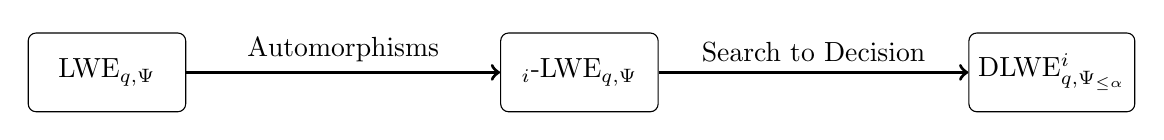
\begin{tikzpicture}
% Define the first acronym
	\node[draw, rounded corners=1mm, minimum width=2cm, minimum height=1cm] (A) at (0,0) {LWE$_{q, \Psi}$};

% Define the second acronym
	\node[draw, rounded corners=1mm, minimum width=2cm, minimum height=1cm] (B) at (6,0) {$\q_i$-LWE$_{q, \Psi}$};

% Define the third acronym
	%\node[draw, rounded corners=1mm, minimum width=2cm, minimum height=1cm] (C) at (6,0) {WDLWE$^i_{q, \Psi}$};

% Define the fourth acronym
	%\node[draw, rounded corners=1mm, minimum width=2cm, minimum height=1cm] (D) at (9,0) {DLWE$^i_{q, \D_{\xi}}$};

% Define the fifth acronym
\node [draw, rounded corners=1mm, minimum width=2cm, minimum height=1cm] (E) at (12,0) {DLWE$^i_{q, \Psi_{\leq \alpha}}$};

% Draw the arrows between the acronyms
	\draw[->, very thick] (A.east) -- node [above] {Automorphisms} (B.west);
	%\draw[->, very thick] (B.east) -- node [above] {(2)} (C.west);
	%\draw[->, very thick] (C.east) -- node [above] {(3)} (D.west);
	\draw[->, very thick] (B.east) -- node [above] {Search to Decision} (E.west);
\end{tikzpicture}
\caption{Schematic of reductions from $R$-LWE to $R$-DLWE}
\label{fig:4reds}
\end{figure}

\paragraph{What do we mean by ``act transitively''?}
Although not present in the original, we now explain the implicit details of the proof below. Most importantly, what do we mean by ``act transitively'' and why it is the case.

Recall from section \ref{ant} that the Galois group of a cyclotomic number field $\Q(\zeta_m)$ is isomorphic to $\Z_m^* = \{k: 1 \leq l < m, \gcd(l,m) = 1\}.$ For our choice of $q \equiv 1 \mod m = 2n = 2^k$, this group is actually just
\[ \Z_m^* = \{l \in \Z : l < 2^k, \gcd(l,2^k) = 1 \} = \{l < 2n: l \text{ is odd}\}, \]
the set of odd integers less than $2n$. When counted, there are precisely $n$ of them. The elements of the group are automorphisms $\tau_i$ such that $\tau_i(\zeta) = \zeta^i$ and the elements of $\Q$ are fixed. Note that, thanks to that isomorphism, we have $\tau_i^{-1} = \tau_{i^{-1}}$.

Let us look now at the $q$ and denote by $\Z_q = \Z_q^*$ the group modulo $q$ under multiplication. Since we picked $q \equiv 1 \mod 2n$ we can take\footnote{The case where $q = c(2n+1)$ for some $c > 1$ is a bit more technical but the following proof works in general for $q = 2n+1$.} for simplicity that $q = 2n + 1$. Then we know that $\varphi(q) = 2n$ -- there are exactly $2n$ integers less than $q$ and coprime with $q$. Therefore there exists some $z \in \Z_q$ such that $z^{2n} \equiv 1 \mod q$ and $z^l \neq 1 \mod q$. Such $z$ is the $2n$-th primitive root of unity modulo $q$. Long time ago, Euler proved that for any prime $q$, there are no nontrivial (i.e. other than 1 and $-1$) square roots modulo $q$. Therefore we must have
\[ z^{2n} \equiv 1 \mod q \implies z^n \equiv -1 \mod q \implies z^n + 1 \equiv 0 \mod q\]
Recall also, from the section about cyclotomic fields, that this means that the set of all conjugates of $z$ are those $z^r$ such that the $\gcd(2n, r) = 1$ which are precisely all the odd integers $< 2n$. Hence, the set
\[ \{z, z^3, z^5, \ldots, z^{2n-1} \} \]
is the set of all the $2n$-th roots of unity and all of those elements are actually in $\Z_q$. We conclude that the polynomial $x^n +1$ ``splits completely'' into linear factors modulo $q$:
\[ x^n + 1 = (x-z)(x-z^3) \cdot \ldots \cdot (x-z^{2n-1}) = \prod_{\substack{r \, <\, 2n \\ r \text{ is odd}}} (x-z^r). \]
By the CRT (Proposition \ref{crt}), there is an isomorphism
\[ R_q = \Z_q[x] \Big/\prod_{\substack{r \, < \, 2n \\ r \text{ is odd}}}(x-z^r) \rightarrow  \Z_q[x]/(x-z) \cross  \Z_q[x]/(x-z^3) \cross \ldots \cross  \Z_q[x]/(x-z^{2n-1})\]

Since our underlying ring is a Dedeking domain (it is a ring of integers) and each $\q_r = (x-z^r)$ is prime (for $a,b$ odd, if $z^a \cdot z^b \in (z^r)$ then either $a$ or $b$ must thus be in $(z^r)$ because a sum of two odd integers is even) for all odd $r < 2n$, they are actually maximal. Therefore, we have $\Z_q[x]/(x-z^r) \cong \Z_q$ -- the field of integers modulo a prime $q$. 

Finally tying those two concepts together (the Galois group and $\Z_q$) notice that each $\tau_i \in \Z_m^*$ will map $z \mapsto z^i$ therefore permuting the corresponding elements in $R_q = \Z_q[x] \Big/\prod_{r \in \Z_m^*}\q_r$ mapping each $\q_r$ to $\tau_i(\q_r) = \q_{r\cdot i^{-1}}$ where the multiplication is performed modulo $q$.

\paragraph{Search to Worst-Case Decision}
We begin with the reduction of the LWE to $\q_i$-LWE distribution relative to only one $\q_i$ arbitrary prime ideal.
\begin{definition}
	The $\q_i$-LWE$_{q,\Psi}$ problem is: given access to A$_{s,\Psi}$ for some arbitrary $s \in R_q$ and $\psi \in \Psi$, find $s \mod \q_i R$.
\end{definition}
\begin{lemma}[LWE to $\q_i$-LWE, Lemma 5.5 \cite{ring-lwe}]
	Suppose that the family $\Psi$ is closed under all the automorphisms of $K$, i.e., $\psi \in \Psi \Rightarrow \tau_k(\psi) \in \Psi$ for every $k \in \Z^*_m$. Then for every $i \in \Z^*_m$, there is a deterministic polynomial-time reduction from LWE$_{q, \Psi}$ to $\q_i$-LWE$_{q, \Psi}$.
\end{lemma}

\begin{proof}
	By assumptions, we are given access to an $\q_i$-LWE oracle along with $n$ field automorphisms $\tau_k$ that ``act transitively'' on the prime ideals $\q_i$ thanks to the underlying field being a cyclotomic number field as explained above. The idea is to use the oracle to recover the value of $s$ relative to every $\q_j R$ using the automorphisms. Once we have that, we can (efficiently) recover the $s$ using the Chinese Remainder Theorem. 

	The reduction to find $s \mod \q_j R$ works as follows: transform each given sample $(a,b) \leftarrow \text{A}_{s, \psi}$ to $(\tau_k(a), \tau_k(b)) \in R_q \cross R_q$ where $k = j \cdot i^{-1} \in \Z^*_m$ which gives $\tau_k(\q_j) = \q_i$. Give the transformed sample to the oracle which outputs some $t \in R / \q_i R$. Since $\tau_k$ is a bijection, we can compute $\tau^{-1}_k(t) \in R / \q_j R$.

	We now need to verify that this output is actually equal to $s \mod \q_j R$. This is equivalent to asking if $(\tau_k(a), \tau_k(b))$ is distributed according to A$_{\tau_k(s), \psi '}$ for $\psi ' = \tau_k(\psi)$. First, note that the automorphisms fix the underlying structure. Namely, $\tau_k(R) = R$ and in particular, $\tau_k(q) = q$ for any $k \in \Z_m^*$. We therefore have
	\[ \tau_k(b) = \tau_k(a)\cdot \tau_k(s) + \tau_k(e).\]
	If $a$ was uniformly distributed, $\tau_k(a)$ will be as well. The pairs are therefore distributed according to A$_{\tau_k(s), \psi '}$ for $\psi ' = \tau_k(\psi) \in \Psi$. The $t$ returned by an oracle must therefore be $t = \tau_k(s) \mod \q_i R$ and so $\tau_k^{-1}(t) = s \mod \tau_k^{-1}(\q_i R) = s \mod \q_j R$ as required. 

	All we need to show now is that the automorphisms preserve the distribution. Note that since the automorphisms simply permute the coordinates of the canonical embedding (see Section \ref{ant}), then for any $\psi = \D_{\bm{r}} \in \Psi_{\leq \alpha}$ (each $r_i$ of the vector $\bm{r}$ is $\leq \alpha$) and any $\Q$-automorphism $\tau_k: K \rightarrow K$, we have $\tau_k(\D_{\bm{r}}) = \D_{\bm{r'}}$ where $\bm{r'}$ is just a permutation of the coordinates of $\bm{r}$ and so each $r_i$ is still $\leq \alpha$.

\end{proof}
We ilustrate how the automorphisms act on the ring with the following example.
\begin{example}
	Take $n = 2$ and $q = 2n+1 = 5$. The ring now looks like $R_q := \Z_q[x]/\Phi_{2n}(x) = \Z_5[x]/(x^2+1)$. Since $z = 2$ is the primitive root modulo 5, our polynomial splits as $x^2+1 \mod 5 \equiv (x-2)(x-2^3) \equiv (x-2)(x-3)$. So our ideals are $\q_1 = (x-2)$ and $\q_2 = (x-3)$.

	Just like in the proof, we are given access to an oracle -- call it $\orc$ (in this case we will act as one because we already know the secret $s$, in principle, we need $\orc$ to be efficient for the reduction to work) -- that yields $s(x)$ modulo only one ideal, say it will be $\q_1$ in this example.

	Let us now take $s(x), a(x) \in \Z_5[x]/(x^2+1)$ to be $s(x) = 1 + 4x$ and $a(x) = 2x$. Since the oracle $\orc$ will return us the correct result for any input, it will also return us the correct input when the error $e$ is 0. Let us then take it as such.

	So we now encounter a sample $(a,b) \leftarrow A_{s, \psi}$ that looks like 
	\[ (a, a\cdot s + e) = (2x, 2x(1+4x)) = (2x, 2x +8x^2) = (2x, 2+2x). \]
	Let us give this sample to $\orc$ which will tell us what is $s(x) \mod \q_1 R_q$. Since we are the oracle, we need to do the computation, and so
	\[ s(x) \mod (x-2)R_q = 4 \]
	is the answer.

	Compute now $b \mod \q_3 R_q = 2 +2x \mod (x-3)R_q = 3$ so that we can use the automorphism $\tau_k = \tau_{j/i} = \tau_3$ to map it to the result modulo $\q_1$ for which we can obtain the answer. Note that we in fact can compute this because the $q$ is known to everyone. Only the secret $s$ and the distribution $\psi$ are unknown, all the other variables are public. We therefore have
	\[ \tau_3(2+2x) = 2 +2x^3 = 2 -2x = 2+3x \]
	and $\orc$ responds with $2+3x \mod q_1 R_q = 3$. We now map $3(x-3)$ using $\tau_3^{-1} = \tau_{3^{-1}} = \tau_2$:
	\[ \tau_2(3(x-3)) = \tau(3x-9) = \tau_2(3x+1) = 3x^2 + 1 = -3 +1 = 3. \]

	Since we exhausted all the automorphisms (there are only 2), we can finally use the Chinese Remainder Theorem on the following system of equations where we set $s(x) = \alpha x + \beta$ as the intermediate values:
	\begin{align*} & \begin{cases}
		\alpha x + \beta = 4 \mod (x-2)R_q \\
		\alpha x + \beta = 3 \mod (x-3)R_q
	\end{cases} \implies 
	\begin{cases} 
		2 \alpha + \beta = 4 \\
		3 \alpha + \beta = 3
	\end{cases} \\
				   & \beta = 4 - 2 \alpha \implies 3 \alpha + 4 - 2 \alpha = 3 \implies \alpha = 4 \\
				   & \implies \beta = 4-2\cdot 4 = 1
\end{align*}
So $s(x) = \alpha x + \beta = 4x + 1$ which is (unsurprisingly) the correct answer.	
\end{example}
\iffalse
\begin{example}
	As the second example, take $n = 8$ and $q = 2n+1 = 17$. Set $a,s \in \Z_17[x]/(x^8+1)$ as $a = x^2 + 16x^7$ and $s = 1 + x + 2x^2$. Just like in the previous example, we will take $e=0$ and we compute:
	\begin{align*}
		a\cdot s & = (x^2+16x^7)(1+x+2x^2) \\
				 & = x^2 + x^3 + 2x^4 + 16x^7 + 16x^8 +32x^9 \\
				 & = 1 + 2x +x^2 +x^3+2x^4+16x^7
	\end{align*}
	The primitive root modulo 17 is 3 and so $x^8+1 \mod 17$ splits as $x^n+1 = \q_1 \cdot \q_3 \cdot \ldots \cdot \q_{13} \cdot \q_{15}$ where each $\q_r = (x-z^r) = (x-3^r)$ giving:
	\begin{align*}
		& \q_1 = (x-3) & \q_9 & = (x-14) \\
		& \q_3 = (x-10) & \q_{11} & = (x-7) \\
		& \q_5 = (x-5) & \q_{13} & = (x-12) \\
		& \q_7 = (x-11) & \q_{15} & = (x-6)
	\end{align*}

\end{example}
\fi

The last step left for us is the reduction to the decision-RLWE. We will define some notation first. For convenience, we will identify the elements of $\Z_m^*$ with their integer representatives from the set $\{1, \ldots, m-1\}$ with the usual ordering. For $i \in \Z_m^*$ we let $i-$ denote the largest element in $\Z_m^*$ less than $i$, defining $1-$ to be 0.
\begin{definition}[Hybrid LWE distribution]
	For $i \in \Z_m^*, s \in R_q$, and a distribution $\Psi$ over $R_q$, the
	distribution $A^i_{s,\Psi}$ over $R_q \cross R_q$ is defined as follows: choose $(a, b) \leftarrow A_{s, \Psi}$ and output $(a, b + h/q)$ where $h \in R_q$ is uniformly random and independent$\mod \q_j R_q$ for all $j \leq i$, and is $0 \mod$ all the remaining $\q_j R_q$. Also define $A^0_{s,\Psi}$ simply as $A_{s,\Psi}$.
\end{definition}
\begin{definition}
  For $i \in \Z_m^*$ and a family of distributions $\Psi$, the DLWE$^i_{q,\Psi}$ problem is defined as follows: given access to $A^j_{s,\Psi}$ for arbitrary $s \in \R_q$, $\psi \in \Psi$, and $j \in \{i$-$, i\}$, find $j$.
\end{definition}
\begin{lemma}[$\q_i$-LWE to DLWE$^i$]
  For any $i \in \Z_m^*$, there is a reduction from $\q_i$-LWE$_{q, \Psi}$ to DLWE$^{\text{ }i}_{q, \Psi}$.
\end{lemma}
\begin{proof}
  Let us present a transformation alike the one given in Lemma \ref{s-to-d}. When given some $g \in R_q$, we will map it to either $A^{i\text{-}}_{s, \psi}$ or $A^i_{s, \psi}$ depending on whether or not $f = s \mod \q_i$ (note that thanks to our definition the values modulo the other $\q_jR$ are irrelevant). The transformation works as follows: given a sample $(a, b) \leftarrow A_{s, \psi}$, output a sample
  \[ (a', b') = (a +v, b+h+vg) \in R_q \cross R_q \]
  where $v \in R_q$ is uniformly random$\mod \q_i$ and is 0 modulo the other $\q_j$'s, and $h \in \R_q$ is uniformly random and independent$\mod \q_j R$ for all $j < i$, and is 0$\mod$ all the other remaining $\q_j R$. We first note that since both $a$ and $v$ are uniformly random, so is $a'$. Next, we fix the $a'$ and consider what happens with $b'$ which can be written as
  \[ \begin{split}b' \; = \; b + h+vg \; \; = & \; \; as +h +vg +e \\
    & \; \; a's +h +v(g-s) +e
  \end{split}\]
  where the $e$ is taken from our distribution $\psi$.

  Let us consider two cases.
  \begin{enumerate}
    \item $g$ is in fact equal to $s \mod \q_i R$. Then by the CRT, $v(g-s) = 0 \in R_q$ and so the distribution of $(a', b')$ is precisely $A^{i-}_{s, \psi}$.
    \item $g \neq s \mod \q_i R$. Since $\q_i$ is a maximal ideal, $R/\q_i$ is a field and so the $v(g-s) \in R_q$ is distributed uniformly$\mod \q_i R$ for all $j \leq i$, and is 0 modulo all the other remaining $\q_j R$. Therefore the distribution of $(a', b')$ is exactly $A^i_{s, \psi}$ as required.
  \end{enumerate}
\end{proof}

\paragraph{Alternative proof}
There is great disparity between required assumptions for the search and the decision version of the problem. The former holds for any number ring, (not even cyclotomic) whereas we need to make many assumptions about the structure of the ring from which we sample our variables from. It would be very practical if we could attain the same results but for more general structure. For one, the Galois fields are rare to encouter and the application might require us to consider something more modest. Secondly, from the cryptoanalytical point of view, usually the more assumptions we make, the less secure our problem is in the sense that one could abuse the additional structure for a specified attack.

One of the solutions was presented by C.Peikert O. Regev and N. Stephens-Davidowitz in their 2020 paper \textit{Pseudorandomness of Ring-LWE for Any Ring and Modulus} -- \cite{oracle}. The approach they use differs greately from the one we introduced here. Firstly, the reduction is from the decision-RLWE to the \prob{BDD} (which was replaced by \prob{CVP} in our case) directly, without invoking an oracle for the search version at all. Secondly, as mentioned, this reduction works for any number field $K$, not only cyclotomic, as well as for any modulus $q$, not only prime.

The very brief description of their approach is as follows. We take a point $t$ from the ambient space and use the decision oracle to measure how close it is to the actual lattice point. The goal is to use the so called ``acceptance probability'' of the oracle on some new point, call it $t'$, and check if it is significantly closer to the desired solution. This approach seems to be very easy, however, there are many important questions that need to be answered before proving that it actually works. For example, how do we pick the point $t'$ and, more importantly, how do we know it is in fact closer to the desired solution? Answering the second question is the main concern of the paper. For the full proof, the reader is redirected to the paper itself -- \cite{oracle}.
